\documentclass[a4paper,12pt]{article}
%%%%%%%%%%%%%%%%%%%%%%%%%%%%%%%%%%%%%%%%%%%%%%%%%%%%%%%%%%%%%%%%%%%%%%%%%%%%%%%%%%%%%%%%%%%%%%%%%%%%%%%%%%%%%%%%%%%%%%%%%%%%%%%%%%%%%%%%%%%%%%%%%%%%%%%%%%%%%%%%%%%%%%%%%%%%%%%%%%%%%%%%%%%%%%%%%%%%%%%%%%%%%%%%%%%%%%%%%%%%%%%%%%%%%%%%%%%%%%%%%%%%%%%%%%%%
\usepackage{eurosym}
\usepackage{vmargin}
\usepackage{amsmath}
\usepackage{graphics}
\usepackage{epsfig}
\usepackage{subfigure}
\usepackage{fancyhdr}
%\usepackage{listings}
\usepackage{framed}
\usepackage{graphicx}

\setcounter{MaxMatrixCols}{10}
%TCIDATA{OutputFilter=LATEX.DLL}
%TCIDATA{Version=5.00.0.2570}
%TCIDATA{<META NAME="SaveForMode" CONTENT="1">}
%TCIDATA{LastRevised=Wednesday, February 23, 2011 13:24:34}
%TCIDATA{<META NAME="GraphicsSave" CONTENT="32">}
%TCIDATA{Language=American English}

\pagestyle{fancy}
\setmarginsrb{20mm}{0mm}{20mm}{25mm}{12mm}{11mm}{0mm}{11mm}
\lhead{MA4128} \rhead{Kevin O'Brien}
\chead{Logistic Regression}
%\input{tcilatex}


\begin{document}

%\tableofcontents


\section*{Logistic Regression}
\begin{itemize}
	\item Logistic regression determines the impact of multiple independent variables
	presented simultaneously to predict membership of one or other of the two
	dependent variable categories.
	\item 
	A range of regression techniques have been developed for analysing data with categorical dependent
	variables, including logistic regression and discriminant analysis.
\end{itemize}




There are two main uses of logistic regression:
\begin{itemize}
	\item The first is the prediction of group membership. Since logistic regression calculates the
	probability of success over the probability of failure, the results of the analysis are in
	the form of an \textbf{odds ratio}.
	\item Logistic regression also provides knowledge of the relationships and strengths among
	the variables (e.g. playing golf with the boss puts you at a higher probability for job
	promotion than undertaking five hours unpaid overtime each week).
\end{itemize}




\section*{Introduction to Logistic Regression}
\begin{itemize}
	\item Logistic regression or logit regression is a type of probabilistic statistical classification model.
\item Logistic regression  operates over real-valued vector inputs. 
	
%	The dimensions of the input vectors being classified are called "features" and there is no restriction against them being correlated. 
%	
%	Logistic regression is one of the best probabilistic classifiers, measured in both log loss and first-best classification accuracy across a number of tasks.
%	
%	Logistic regression requires extensive tuning in the form of feature selection and implementation to achieve state-of-the-art classification performance.
	
	\item Logistic regression is also used to predict a binary response from a binary predictor, used for predicting the outcome of a categorical dependent variable (i.e., a class label) based on one or more predictor variables (features). 
	
	\item That is, it is used in estimating empirical values of the parameters in a qualitative response model. The probabilities describing the possible outcomes of a single trial are modeled, as a function of the explanatory (predictor) variables, using a logistic function. 
	
	\item Logistic regression, also called a logit model, is used to model \textbf{dichotomous (i.e. Binary) outcome variables}. In the logit model the log odds of the outcome is modeled as a linear combination of the predictor variables.
	
	\item 
	Binary Logistic regression is used to determine the impact of multiple independent variables
	presented simultaneously to predict membership of one or other of the two
	dependent variable categories.

	\item However, if your dependent variable was not measured on a dichotomous scale, but a continuous scale instead, you will need to carry out \textbf{multiple regression}, whereas if your dependent variable was measured on an ordinal scale, \textbf{ordinal regression} would be a more appropriate starting point.
\end{itemize}


\subsection*{Examples of Logistic Regression}

\begin{description}
	\item[Example 1:]  Suppose that we are interested in the factors that influence whether a political candidate wins an election.  The outcome (response) variable is binary (0/1); \textit{ win or lose}.  The predictor variables of interest are the amount of money spent on the campaign, the amount of time spent campaigning negatively and whether or not the candidate is an incumbent.
	
	\item[Example 2:]  A researcher is interested in how variables, such as GRE (Graduate Record Exam scores), GPA (grade point average) and prestige of the undergraduate institution, effect admission into graduate school. The response variable, \textit{admit/don't admit}, is a binary variable.
\end{description}


\subsection*{The Purpose of Logistic Regression}
\begin{itemize}
	\item The crucial limitation of linear regression is that it cannot deal with Dependent Variables’s that are \textbf{\textit{dichotomous}} and categorical. 
	\item Many interesting variables in the business world are dichotomous: for
	example, consumers make a decision to buy or not buy (\textit{\textbf{Buy/Don't Buy}}), a product may pass or fail quality control (\textit{\textbf{Pass/Fail}}), there are good or poor credit risks (\textit{\textbf{Good/Poor}}), an employee may be promoted or not (\textit{\textbf{Promote/Don't Promote}}).
	

	
	\item 	Logistical regression is regularly used rather than discriminant analysis when there are only two categories
	for the dependent variable. Logistic regression is also easier to use with SPSS than discriminant analysis when
	there is a mixture of numerical and categorical Independent Variables’s, because it includes procedures for
	generating the necessary dummy variables automatically, requires fewer assumptions, and
	is more statistically robust. 
	
	\item Discriminant analysis strictly requires the continuous independent variables  (though dummy variables can be used as in multiple regression). Thus, in instances where
	the independent variables are categorical, or a mix of continuous and categorical, and the
	Dependent Variable is categorical, logistic regression is necessary.
\end{itemize}



\subsection*{Use of Binomial Probability Theory}
\begin{itemize}
	\item Since the dependent variable is dichotomous we cannot predict a numerical value for it
	using logistic regression, so the usual regression least squares deviations criteria for best fit
	approach of minimizing error around the line of best fit is inappropriate.
	
	\item 	Instead, logistic regression employs binomial probability theory in which there are only two values to
	predict: that probability (p) is 1 rather than 0, i.e. the event/person belongs to one group
	rather than the other.
	\item Logistic regression forms a best fitting equation or function using the
	maximum likelihood method (not part of course), which maximizes the probability of classifying the observed
	data into the appropriate category given the regression coefficients.
\end{itemize}



\subsection{Assumptions of logistic regression}
\begin{itemize}
\item Logistic regression does not assume a linear relationship between the dependent and
independent variables.
\item The dependent variable must be a dichotomy (2 categories).
(Remark: Dichotomous refers to two outcomes. Multichotomous refers to more than two outcomes).
\item The independent variables need not be interval, nor normally distributed, nor linearly
related, nor of equal variance within each group.
\item The categories (groups) must be mutually exclusive and exhaustive; a case can only be
in one group and every case must be a member of one of the groups.
\item Larger samples are needed than for linear regression because maximum likelihood
coefficients are large sample estimates. A minimum of 50 cases per predictor is
recommended.
\end{itemize}
\newpage
\subsection*{Exercise Data Set}
The exercise data set comes from a survey of home owners
conducted by an electricity company about an offer of roof solar panels with a 50\% subsidy
from the state government as part of the state’s environmental policy. The variables involve
household income measured in units of a thousand dollars, age, monthly mortgage, size of
family household, and as the dependent variable, whether the householder would take or decline the offer.
The purpose of the exercise is to conduct a logistic regression to determine whether family
size and monthly mortgage will predict taking or declining the offer.

\subsection*{Exercise}
\begin{itemize}
	\item For the first demonstration, we will use `family size’ and
	`mortgage’ only. 
	\item For the options, select Classification Plots, Hosmer-Lemeshow Goodness
	Of Fit, Casewise Listing Of Residuals and select Outliers Outside 2sd. 
		\item 
	Retain default
	entries for probability of stepwise, classification cutoff and maximum iterations.
\end{itemize}


\begin{figure}[h!]
\begin{center}
  % Requires \usepackage{graphicx}
  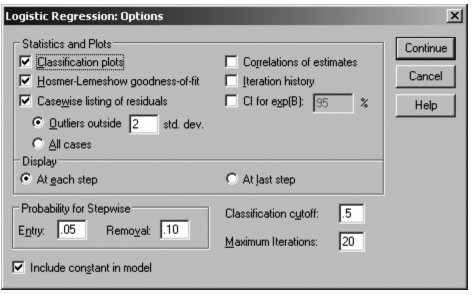
\includegraphics[scale=0.8]{images/Logistic10}\\
  \caption{Selected Options for Exercises}
\end{center}
\end{figure}

We are not using any categorical variables this time. If there are categorical variables, use the \textbf{\textit{categorical}} option. For most situations, choose the ‘indicator’ coding scheme (it is the
default).
\subsection{SPSS Outout  - Block 0: Beginning Block.}
Block 0 presents the results with only the constant included
before any coefficients (i.e. those relating to family size and mortgage) are entered into
the equation. Logistic regression compares this model with a model including all the
predictors (family size and mortgage) to determine whether the latter model is more
appropriate. The table suggests that if we knew nothing about our variables and guessed
that a person would not take the offer we would be correct 53.3\% of the time.
\begin{figure}[h!]
\begin{center}
  % Requires \usepackage{graphicx}
  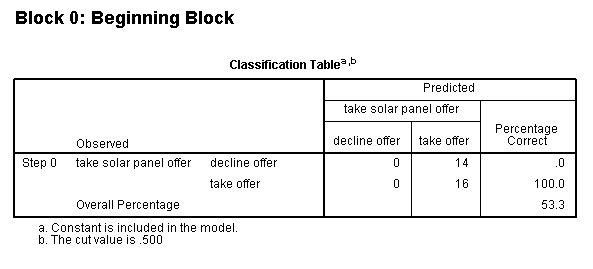
\includegraphics[scale=0.6]{images/Logistic3}\\
  \caption{Classification table}
\end{center}
\end{figure}
The variables not in the equation table tells us whether each IV improves the model. The answer is yes for both variables, with family size slightly better than mortgage size, as both are significant and if included would add to the predictive power of the model. If they had not been significant and able to contribute to the prediction,
then termination of the analysis would obviously occur at this point

\begin{figure}
\begin{center}
  % Requires \usepackage{graphicx}
  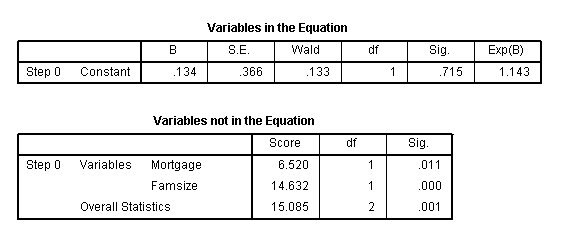
\includegraphics[scale=0.6]{images/Logistic4}\\
  \caption{Variables in / not in the equation}
\end{center}
\end{figure}
This presents the results when the predictors ‘family size’ and
‘mortgage’ are included. Later SPSS prints a classification table which shows how the
classification error rate has changed from the original 53.3\%. By adding the variables
we can now predict with 90\% accuracy (see Classification Table later). The
model appears good, but we need to evaluate model fit and significance as well. SPSS will
offer you a variety of statistical tests for model fit and whether each of the independent
variables included make a significant contribution to the model.
\begin{figure}
\begin{center}
  % Requires \usepackage{graphicx}
  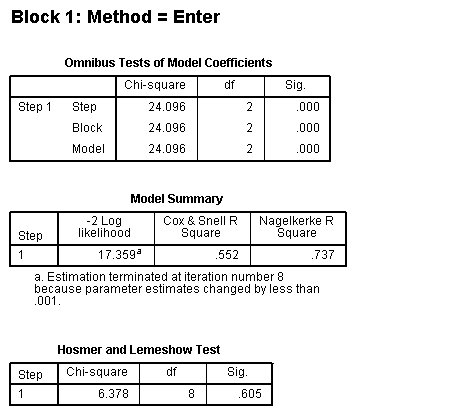
\includegraphics[scale=0.6]{images/Logistic5}\\
  \caption{Test Outcomes}
\end{center}
\end{figure}






\section*{Introduction to Logistic Regression}

The term ‘\textbf{\textit{generalized linear model}}’ is used to describe a procedure for
transforming the dependent variable so that the ‘right hand side’ of the model
equation can be interpreted as a \textbf{‘\textit{linear combination}}’ of the explanatory variables. 	In logistic regression, the logit may be computed in a manner similar to linear regression:
\[ \eta_i = \beta_0 + \beta_1x_1 + \beta_2x_2 + \ldots  \]

In situations where the dependent (y) variable is continuous and can be
reasonably assumed to have a normal distribution we do not transform the y
variable at all and we can simply run a multiple linear regression analysis.

Otherwise some sort of transformation is applied.


%---------------------------------------------------------------%
\subsection{Binomial Logistic Regression} 
A binomial logistic regression (often referred to simply as logistic regression), predicts the probability that an observation falls into one of two categories of a \textbf{dichotomous} dependent variable based on one or more independent variables that can be either continuous or categorical.

% \section{Binomial Logistic Regression}
Binomial logistic regression estimates the probability of an event (as an example, having heart disease) occurring. 
\begin{itemize}
	\item If the estimated probability of the event occurring is greater than or equal to 0.5 (better than even chance), the procedure classifies the event as occurring (e.g., heart disease being present). \item If the probability is less than 0.5, Logistic regression classifies the event as not occurring (e.g., no heart disease). 
\end{itemize}


\section{Review of Logistic Regression}
% http://www.nesug.org/proceedings/nesug06/an/da26.pdf
% http://www.ccsr.ac.uk/publications/teaching/blr.pdf
% http://www.southampton.ac.uk/ghp3/docs/unicef/presentation7.1a.pdf
% ftp://public.dhe.ibm.com/software/analytics/spss/documentation/statistics/20.0/en/client/Manuals/IBM_SPSS_Regression.pdf
% http://www.umass.edu/statdata/statdata/data/


%---------------------------------------------------------------%
\subsection{Logistic Regression}
Logistic regression or logit regression is a type of regression analysis used for predicting
the outcome of a categorical dependent variable (a dependent variable that can take on a limited number of values,
whose magnitudes are not meaningful but whose ordering of magnitudes may or may not be meaningful)
based on one or more predictor variables.



\begin{itemize}
	\item[1.)] Logistic regression is intended for the modeling
	of dichotomous categorical outcomes (e.g., characterized by binary responses: buy vs Don't buy, dead vs. alive, cancer vs. none,…).
	
	
	\item[2.)] We want to predict the probability of a particular response  (0 to 1 scale).
	
	\item[3.)] For binary responses, linear regression should not be used for several reasons
	but the most common-sense reason is that linear regression can provide predictions NOT on a 0 to 1 scale.
	but rather a predicted response of some numeric value (e.g 2.4 or -800.3).
	
	\item[4.)] We need a way to link the probabilistic response variable to the continuous and/or categorical predictors and
	keep things on this 0 to 1 scale.
	
	\item[5.)] Logistic regression winds up transforming the probabilities to odds and then taking the natural logarithm of these odds, called logits.
	
	
	\item[6.)] Suppose a response variable is passing a test (by convention, 0=no and 1=yes).
	You have 1 predictor - number of days present in class over the past 30 days.
	Suppose the regression coefficient (often just called beta) in the output is .14.
	You would then say that, on average, as class presence increases by 1 day, the natural logarithm of the
	odds of passing the test increases by .14.
	
	\item[7.)] For the interpretation, you can just talk about the odds.
	Most computer output will give you this number.
	Suppose the answer in odds is 1.24. Then, you just say that,on average, as class presence increases by 1 day,
	the odds of passing the test are multiplied by 1.24.
	In other words, for each additional day present, the odds of passing are 24% greater than that of not passing.
	
	\item[8.)] To validate our findings, normally, we test whether the regression coefficient is equal to zero in the population.
	In logistic regression, the corresponding value for the odds is one (not zero). We got an odds of 1.24.
	Can we trust this? Or should we go with one (which would mean that the odds are the same for both passing and not passing,
	and hence class presence makes no difference at all)?  Look at the p-value (significance). If it less than .05 (by convention), you have enough evidence to reject
	the notion that the odds are really one. You go ahead and support the 1.24 result.
\end{itemize}

\end{document}
